\documentclass[aspectratio=169,10pt]{beamer}

\usepackage[utf8]{inputenc}
\usepackage[T1]{fontenc}

\usetheme{Madrid}
\usecolortheme{seahorse}

\usepackage{amsmath}
\usepackage{amssymb}
\usepackage{mathtools}
\usepackage{xcolor}
\usepackage{listings}
\usepackage{graphicx}
\usepackage{hyperref}

\graphicspath{{figures/}}

% Python style for code
\lstdefinestyle{python}{
    language=Python,
    basicstyle=\ttfamily\scriptsize,
    commentstyle=\color{green!50!black}\itshape,
    keywordstyle=\color{blue}\bfseries,
    stringstyle=\color{red},
    numbers=left,
    numberstyle=\tiny\color{gray},
    frame=single,
    breaklines=true,
    showstringspaces=false,
    tabsize=4
}

% Setup footline
\setbeamertemplate{footline}[frame number]

% Title and Author
\title{Chapter 8: Convex Functions}
\subtitle{Convex Analysis and Monotone Operator Theory in Hilbert Spaces}
\author{Bauschke \& Combettes (2017)}
\date{\today}

\begin{document}

\frame{\titlepage}

% ============================================================================
% TABLE OF CONTENTS
% ============================================================================

\begin{frame}[fragile]{Chapter 8: Convex Functions}
    \tableofcontents
\end{frame}

% ============================================================================
% SECTION 1: BASIC PROPERTIES AND EXAMPLES
% ============================================================================

\section{Basic Properties and Examples}

\begin{frame}[fragile]{Convex Functions: Definitions}
    \textbf{Definition 8.1:} A function $f : \mathcal{H} \to [-\infty, +\infty]$ is \textit{convex} if
    \[
    f(\alpha x + (1-\alpha) y) \leq \alpha f(x) + (1-\alpha) f(y)
    \]
    for all $x, y \in \text{dom} f$ and $\alpha \in [0,1]$.

    \vspace{0.3cm}

    \textbf{Definition 8.7:} $f$ is \textit{strictly convex} if
    \[
    x \neq y \implies f(\alpha x + (1-\alpha) y) < \alpha f(x) + (1-\alpha) f(y)
    \]
    for all $x, y \in \text{dom} f$ and $\alpha \in (0,1)$.

    \vspace{0.3cm}

    \textbf{Key Concept:} The epigraph $\text{epi} f = \{(x,r) \in \mathcal{H} \times \mathbb{R} : f(x) \leq r\}$ 
    is convex \textit{if and only if} $f$ is convex.
\end{frame}

\begin{frame}[fragile]{Jensen's Inequality}
    \textbf{Proposition 8.11:} Let $f : \mathcal{H} \to [-\infty, +\infty]$ be convex. Then
    \[
    f\left(\sum_{i \in I} \alpha_i x_i\right) \leq \sum_{i \in I} \alpha_i f(x_i)
    \]
    for all finite families $(\alpha_i)_{i \in I}$ in $[0,1]$ with $\sum_{i \in I} \alpha_i = 1$ and $(x_i)_{i \in I}$ in $\text{dom} f$.

    \vspace{0.3cm}

    \textbf{Corollary 8.12:} For convex $f$: if $(x_i)_{i \in I}$ are in $\text{dom} f$ with weights $(\alpha_i)_{i \in I}$ 
    summing to 1, then Jensen's inequality holds.

    \vspace{0.3cm}

    \textit{Interpretation:} The function value at a weighted average is at most the weighted average of function values.
\end{frame}

\begin{frame}[fragile]{Examples: Basic Convex Functions}
    \textbf{Example 8.9:} The norm $\| \cdot \| : \mathcal{H} \to \mathbb{R}$ is convex:
    \[
    \|\alpha x + (1-\alpha) y\| \leq \alpha \|x\| + (1-\alpha)\|y\|
    \]
    but \textit{not strictly convex} (e.g., take $x = -y$).

    \vspace{0.3cm}

    \textbf{Example 8.10:} The squared norm $\| \cdot \|^2 : \mathcal{H} \to \mathbb{R}$ is \textit{strictly convex}.
    Proof: By Corollary 2.15 (parallelogram law).

    \vspace{0.3cm}

    \textbf{Example 8.19:} For a bounded sequence $(z_n)_{n \in \mathbb{N}}$ in $\mathcal{H}$:
    \[
    f : \mathcal{H} \to \mathbb{R}, \quad f(x) = \limsup_{n \to \infty} \|x - z_n\|
    \]
    is convex and Lipschitz continuous with constant 1.
\end{frame}

\begin{frame}[fragile]{Convex Functions on Subsets}
    \textbf{Definition:} Let $C$ be a nonempty subset of $\text{dom} f$. Then $f$ is \textit{convex on} $C$ if
    \[
    (\forall x, y \in C)(\forall \alpha \in [0,1]) \quad f(\alpha x + (1-\alpha)y) \leq \alpha f(x) + (1-\alpha)f(y)
    \]

    \vspace{0.3cm}

    \textbf{Remark 8.8:} $f + \iota_C$ is convex if and only if $C$ is convex and $f$ is convex on $C$.

    \vspace{0.3cm}

    \textbf{Corollary 8.5:} For convex $f : \mathcal{H} \to [-\infty, +\infty]$ and every $\xi \in \mathbb{R}$:
    \[
    \text{lev}_\xi f := \{x \in \mathcal{H} : f(x) \leq \xi\}
    \]
    is a convex set.
\end{frame}

\begin{frame}[fragile]{Convexity and Differentiability}
    \textbf{Proposition 8.14:} Let $\phi : \mathbb{R} \to [-\infty, +\infty]$ be differentiable on a nonempty open interval $I$ 
    in $\text{dom} \phi$. Then:
    
    \begin{enumerate}
        \item If $\phi'$ is increasing on $I$, then $\phi$ is convex on $I$.
        \item If $\phi'$ is strictly increasing on $I$, then $\phi$ is strictly convex on $I$.
    \end{enumerate}

    \vspace{0.3cm}

    \textit{Intuition:} Increasing derivative $\Rightarrow$ increasing slope $\Rightarrow$ convex function.
\end{frame}

\begin{frame}[fragile]{Convex Function Examples from Calculus}
    \textbf{Example 8.15:} Let $\psi : \mathbb{R} \to \mathbb{R}$ be increasing and $\alpha \in \mathbb{R}$. Define
    \[
    \phi : \mathbb{R} \to [-\infty, +\infty], \quad \phi(x) = \begin{cases}
        \int_\alpha^x \psi(t) dt & \text{if } x \geq \alpha \\
        +\infty & \text{otherwise}
    \end{cases}
    \]
    
    Then $\phi$ is convex. If $\psi$ is strictly increasing, then $\phi$ is strictly convex.

    \vspace{0.3cm}

    \textbf{Example 8.22:} For continuous increasing $\psi : \mathbb{R} \to \mathbb{R}$ with $\psi(0) \geq 0$:
    \[
    f : \mathcal{H} \to \mathbb{R}, \quad f(x) = \int_0^{\|x\|} \psi(t) dt
    \]
    is convex. If $\psi$ is strictly increasing, $f$ is strictly convex.
\end{frame}

\begin{frame}[fragile]{Power Functions and $p$-norms}
    \textbf{Example 8.23:} For $p \in [1, +\infty)$, the function $\| \cdot \|^p$ is strictly convex:
    \[
    (\forall x, y \in \mathcal{H}) \quad \|x + y\|^p \leq 2^{p-1}(\|x\|^p + \|y\|^p)
    \]

    \vspace{0.3cm}

    \textbf{Example 8.31:} The Rényi divergence between $x = (\xi_i)_{i \in I} \in \mathbb{R}_+^N$ 
    and $y = (\eta_i)_{i \in I} \in \mathbb{R}_+^N$ is:
    \[
    f(x,y) = \begin{cases}
        \sum_{i \in I} \xi_i^\alpha \eta_i^{-\alpha} & \text{if } x \in \mathbb{R}_{++}^N, y \in \mathbb{R}_{++}^N \\
        +\infty & \text{otherwise}
    \end{cases}
    \]
    For $\alpha \in [1, +\infty)$, this is convex (apply Example 8.26).
\end{frame}

% ============================================================================
% SECTION 2: CONVEXITY-PRESERVING OPERATIONS
% ============================================================================

\section{Convexity-Preserving Operations}

\begin{frame}[fragile]{Preservation under Supremum and Addition}
    \textbf{Proposition 8.16:} Let $(f_i)_{i \in I}$ be a family of convex functions from $\mathcal{H}$ 
    to $[-\infty, +\infty]$. Then
    \[
    \sup_{i \in I} f_i \text{ is convex}
    \]

    \vspace{0.3cm}

    \textbf{Proposition 8.17:} The set of convex functions from $\mathcal{H}$ to $[-\infty, +\infty]$ is 
    closed under addition and multiplication by strictly positive real numbers.

    \vspace{0.3cm}

    \textbf{Proposition 8.18:} Let $(f_n)_{n \in \mathbb{N}}$ be a sequence of convex functions 
    from $\mathcal{H}$ to $[-\infty, +\infty]$ such that $(f_n)_{n \in \mathbb{N}}$ is pointwise convergent. 
    Then $\lim f_n$ is convex.
\end{frame}

\begin{frame}[fragile]{Composition with Increasing Convex Functions}
    \textbf{Proposition 8.21:} Let $f : \mathcal{H} \to [-\infty, +\infty]$ and $\phi : \mathbb{R} \to [-\infty, +\infty]$ 
    be convex functions. Set $C = \text{conv}(\mathbb{R} \cap \text{ran } f)$ and extend $\phi$ to 
    $\tilde{\phi} : [-\infty, +\infty] \to [-\infty, +\infty]$ by setting $\tilde{\phi}(+\infty) = +\infty$. 
    
    Suppose that $C \subseteq \text{dom} \phi$ and that $\phi$ is increasing on $C$. Then
    \[
    \tilde{\phi} \circ f \text{ is convex}
    \]

    \vspace{0.3cm}

    \textit{Key Example:} If $f$ is convex and $\phi(t) = e^t$, then $e^{f(x)}$ is convex.
\end{frame}

\begin{frame}[fragile]{Integral Functions}
    \textbf{Proposition 8.24:} Let $(\Omega, \mathcal{F}, \mu)$ be a measure space and 
    $\mathcal{H} = L^2((\Omega, \mathcal{F}, \mu); \mathbb{R})$. Let $\varphi : \mathcal{H} \to [-\infty, +\infty]$ 
    be measurable and convex such that
    \[
    (\forall x \in \mathcal{H})(\exists \rho \in L^1((\Omega, \mathcal{F}, \mu); \mathbb{R})) \quad 
    \varphi \circ x \geq \rho \quad \mu\text{-a.e.}
    \]
    
    Then the integral function
    \[
    f : \mathcal{H} \to [-\infty, +\infty], \quad f(x) = \int_\Omega \varphi(x(\omega)) \mu(d\omega)
    \]
    is convex.
\end{frame}

\begin{frame}[fragile]{Perspective Functions}
    \textbf{Definition \& Proposition 8.25:} Let $\varphi : \mathcal{H} \to [-\infty, +\infty]$ be convex, 
    set $C = \{1\} \times \text{epi} \varphi$, and define
    \[
    f : \mathbb{R} \times \mathcal{H} \to [-\infty, +\infty], \quad f(\xi, x) = \begin{cases}
        \xi \varphi(x/\xi) & \text{if } \xi > 0 \\
        +\infty & \text{otherwise}
    \end{cases}
    \]
    
    Then $\text{epi} f = \text{cone } C$ and $f$ is convex.

    \vspace{0.3cm}

    \textit{Application:} This construction shows how to homogenize a convex function.
\end{frame}

\begin{frame}[fragile]{Important Divergences (Examples 8.26--8.31)}
    \textbf{Csiszár $\phi$-divergence:} For convex $\varphi : \mathbb{R} \to [-\infty, +\infty]$,
    \[
    d_\varphi(x,y) = \sum_{i \in I} \eta_i \varphi(\xi_i/\eta_i) \quad \text{is convex in }(x,y)
    \]

    \vspace{0.2cm}

    \textbf{Kullback-Leibler:} $d_{KL}(x,y) = \sum_i \xi_i \ln(\xi_i/\eta_i) - \xi_i + \eta_i$

    \vspace{0.2cm}

    \textbf{Jeffreys:} $d_J(x,y) = \sum_i (\xi_i - \eta_i) \ln(\xi_i/\eta_i)$ 

    \vspace{0.2cm}

    \textbf{Pearson Chi-squared:} $d_P(x,y) = \sum_i (\xi_i - \eta_i)^2 / \eta_i$

    \vspace{0.2cm}

    \textbf{Hellinger:} $d_H(x,y) = \sum_i (\sqrt{\xi_i} - \sqrt{\eta_i})^2$

    \vspace{0.2cm}

    \textbf{Rényi ($\alpha \in [1,+\infty)$):} $d_R(x,y) = \sum_i \xi_i^\alpha \eta_i^{-\alpha}$
\end{frame}

\begin{frame}[fragile]{Marginal and Minkowski Gauge Functions}
    \textbf{Proposition 8.35:} Let $\mathcal{K}$ be a real Hilbert space and $F : \mathcal{H} \times \mathcal{K} \to [-\infty, +\infty]$ 
    be convex. Then the marginal function
    \[
    f : \mathcal{H} \to [-\infty, +\infty], \quad f(x) = \inf_{\mathcal{K}} F(x, \mathcal{K})
    \]
    is convex.

    \vspace{0.3cm}

    \textbf{Definition \& Example 8.36:} The \textit{Minkowski gauge} of a convex set $C$ with $0 \in C$ is
    \[
    m_C : \mathcal{H} \to [-\infty, +\infty], \quad m_C(x) = \inf\{\xi \in \mathbb{R}_{++} : x \in \xi C\}
    \]
    
    This is convex. Moreover: $m_C(0) = 0$ and $m_C(\lambda x) = \lambda m_C(x)$ for $\lambda \in \mathbb{R}_{++}$.
\end{frame}

% ============================================================================
% SECTION 3: TOPOLOGICAL PROPERTIES
% ============================================================================

\section{Topological Properties}

\begin{frame}[fragile]{Lipschitz Continuity of Convex Functions}
    \textbf{Proposition 8.37:} Let $f : \mathcal{H} \to [-\infty, +\infty]$ be proper and convex, 
    let $x_0 \in \text{dom} f$, and let $\rho \in \mathbb{R}_{++}$. Then:
    
    \begin{enumerate}
        \item If $\eta = \sup f(B(x_0; \rho)) < +\infty$ and $\alpha \in [0,1]$, then
        \[
        (\forall x \in B(x_0; \alpha\rho)) \quad |f(x) - f(x_0)| \leq \alpha(\eta - f(x_0))
        \]
        
        \item If $\delta = \text{diam } f(B(x_0; 2\rho)) < +\infty$, then $f$ is Lipschitz continuous 
        relative to $B(x_0; \rho)$ with constant $\delta/\rho$.
    \end{enumerate}

    \vspace{0.3cm}

    \textit{Interpretation:} Convex functions are automatically Lipschitz on bounded sets where they are bounded.
\end{frame}

\begin{frame}[fragile]{Main Continuity Result}
    \textbf{Theorem 8.38:} Let $f : \mathcal{H} \to [-\infty, +\infty]$ be proper and convex, 
    and let $x_0 \in \text{dom} f$. Then the following are equivalent:
    
    \begin{enumerate}
        \item $f$ is locally Lipschitz continuous near $x_0$.
        \item $f$ is continuous at $x_0$.
        \item $f$ is bounded on a neighborhood of $x_0$.
        \item $f$ is bounded above on a neighborhood of $x_0$.
    \end{enumerate}

    \vspace{0.3cm}

    Moreover, if one of these conditions holds, then $f$ is locally Lipschitz continuous on $\text{int dom } f$.

    \vspace{0.3cm}

    \textbf{Intuition:} For convex functions, very weak boundedness assumptions imply strong continuity properties.
\end{frame}

\begin{frame}[fragile]{Continuity in Finite Dimensions}
    \textbf{Corollary 8.40:} Suppose $\mathcal{H}$ is finite-dimensional and $f : \mathcal{H} \to \mathbb{R}$ is convex. 
    Then $f$ is continuous.

    \vspace{0.3cm}

    \textbf{Corollary 8.41:} Suppose $\mathcal{H}$ is finite-dimensional, $f : \mathcal{H} \to [-\infty, +\infty]$ 
    is proper and convex, and $C$ is a nonempty closed bounded subset of $\text{ri dom } f$. 
    Then $f$ is Lipschitz continuous relative to $C$.

    \vspace{0.3cm}

    \textbf{Key Principle:} In finite-dimensional spaces, proper convex functions are always continuous on the 
    relative interior of their domain.
\end{frame}

\begin{frame}[fragile]{Interior of Sublevel Sets}
    \textbf{Proposition 8.46:} Let $f : \mathcal{H} \to [-\infty, +\infty]$. Then:
    
    \begin{enumerate}
        \item If $f$ is upper semicontinuous at $x_0 \in \mathcal{H}$ with $f(x_0) < 0$, then $x_0 \in \text{int } \text{lev}_{\leq 0} f$.
        \item If $f$ is convex and there exists $x_0 \in \mathcal{H}$ with $f(x_0) < 0$, then $\text{int } \text{lev}_{\leq 0} f = \text{lev}_{< 0} f$.
    \end{enumerate}

    \vspace{0.3cm}

    \textbf{Corollary 8.47:} Let $f : \mathcal{H} \to [-\infty, +\infty]$ be convex such that $\text{lev}_{< 0} f \neq \emptyset$. 
    Suppose one of:
    
    \begin{enumerate}
        \item $f$ is upper semicontinuous on $\text{lev}_{< 0} f$.
        \item $f$ is lower semicontinuous and $\text{dom} f$ is open.
        \item $\mathcal{H}$ is finite-dimensional and $\text{dom} f$ is open.
    \end{enumerate}
    
    Then $\text{int } \text{lev}_{< 0} f = \text{lev}_{< 0} f$.
\end{frame}

\begin{frame}[fragile]{The Huber Loss Function}
    \textbf{Example 8.44:} For $\rho \in \mathbb{R}_{++}$, the Huber function is
    \[
    f : \mathbb{R} \to \mathbb{R}, \quad f(x) = \begin{cases}
        \rho|x| - \frac{\rho^2}{2} & \text{if } |x| > \rho \\
        \frac{|x|^2}{2} & \text{if } |x| \leq \rho
    \end{cases}
    \]
    
    Then $f$ is continuous and convex.

    \vspace{0.3cm}

    \textit{Application:} The Huber function is a robust loss function in machine learning that combines 
    quadratic loss (near zero) with linear loss (far from zero).
\end{frame}

\begin{frame}[fragile]{Core of a Convex Function}
    \textbf{Definition:} The \textit{core} of a convex function $f$ is
    \[
    \text{core } f = \{x \in \mathcal{H} : f(x) < +\infty \text{ and } f \text{ is finite on a neighborhood of } x\}
    \]

    \vspace{0.3cm}

    \textbf{Corollary 8.39:} Let $f : \mathcal{H} \to [-\infty, +\infty]$ be proper and convex. 
    Suppose one of:
    
    \begin{enumerate}
        \item $f$ is bounded above on some neighborhood.
        \item $f$ is lower semicontinuous.
        \item $\mathcal{H}$ is finite-dimensional.
    \end{enumerate}
    
    Then $\text{cont } f = \text{int dom } f$.

    \vspace{0.3cm}

    \textit{Interpretation:} Under mild conditions, the "interior of continuity" coincides with the "interior of the domain."
\end{frame}

% ============================================================================
% SECTION 4: NUMERICAL EXAMPLES
% ============================================================================

\section{Numerical Examples and Code}

\begin{frame}[fragile]{Example 1: Convexity Verification in Python}
    \begin{lstlisting}[style=python]
import numpy as np

# Verify Jensen's inequality: f(alpha*x + (1-alpha)*y) <= alpha*f(x) + (1-alpha)*f(y)
def verify_convexity(f, x, y, alpha):
    """Verify Jensen's inequality for function f at points x, y"""
    left_side = f(alpha * x + (1 - alpha) * y)
    right_side = alpha * f(x) + (1 - alpha) * f(y)
    return left_side <= right_side + 1e-10

# Test with f(x) = x^2 (strictly convex)
f = lambda x: x**2
x, y = np.array([1.0, 2.0]), np.array([3.0, 4.0])

for alpha in [0.3, 0.5, 0.7]:
    is_convex = verify_convexity(f, x, y, alpha)
    print(f"alpha={alpha}: Jensen satisfied = {is_convex}")
    \end{lstlisting}

    \vspace{0.2cm}
    Output: All alphas satisfy the inequality with equality when $f$ is strictly convex.
\end{frame}

\begin{frame}[fragile]{Example 2: Kullback-Leibler Divergence}
    \begin{lstlisting}[style=python]
import numpy as np

def kl_divergence(p, q):
    """Kullback-Leibler divergence KL(p || q) = sum(p_i ln(p_i/q_i))"""
    return np.sum(p * np.log(p / q))

def kl_convexity_check(p1, q1, p2, q2, alpha):
    """Check convexity of KL divergence as function of first argument"""
    # Convex combination of distributions
    p_mixed = alpha * p1 + (1 - alpha) * p2
    q_avg = alpha * q1 + (1 - alpha) * q2
    
    left = kl_divergence(p_mixed, q_avg)
    right = alpha * kl_divergence(p1, q1) + (1-alpha) * kl_divergence(p2, q2)
    
    return left <= right + 1e-10

# Test with probability distributions
p1 = np.array([0.2, 0.3, 0.5])
p2 = np.array([0.1, 0.4, 0.5])
q = np.array([0.25, 0.25, 0.5])

alpha = 0.6
is_convex = kl_convexity_check(p1, q, p2, q, alpha)
print(f"KL divergence convexity verified: {is_convex}")
    \end{lstlisting}
\end{frame}

\begin{frame}[fragile]{Example 3: Lipschitz Continuity}
    \begin{lstlisting}[style=python]
import numpy as np

def verify_lipschitz(f, x1, x2, L):
    """Verify Lipschitz continuity: |f(x1) - f(x2)| <= L * ||x1 - x2||"""
    func_diff = abs(f(x1) - f(x2))
    norm_diff = np.linalg.norm(x1 - x2)
    
    return func_diff <= L * norm_diff + 1e-10

# Test with f(x) = ||x|| (Lipschitz with constant 1)
f_norm = lambda x: np.linalg.norm(x)
x1 = np.array([1.0, 2.0, 3.0])
x2 = np.array([1.5, 2.5, 2.5])

L = 1.0  # Lipschitz constant for norm
is_lipschitz = verify_lipschitz(f_norm, x1, x2, L)
print(f"Norm is Lipschitz continuous with L={L}: {is_lipschitz}")

# For bounded region, check ||x||^2
f_squared = lambda x: np.linalg.norm(x)**2
L_bounded = 2 * max(np.linalg.norm(x1), np.linalg.norm(x2))
is_lipschitz_sq = verify_lipschitz(f_squared, x1, x2, L_bounded)
print(f"Squared norm is Lipschitz on bounded region: {is_lipschitz_sq}")
    \end{lstlisting}
\end{frame}

\begin{frame}[fragile]{Example 4: Minkowski Gauge}
    \begin{lstlisting}[style=python]
import numpy as np

def minkowski_gauge(point, convex_set):
    """Compute Minkowski gauge: m_C(x) = inf{lambda > 0 : x in lambda*C}"""
    # For a ball of radius r centered at origin:
    # m_C(x) = ||x|| / r
    
    # For unit ball:
    r_set = 1.0  # radius of convex set
    return np.linalg.norm(point) / r_set

def verify_gauge_homogeneity(x, lambda_val):
    """Verify: m_C(lambda*x) = lambda * m_C(x)"""
    gauge_x = minkowski_gauge(x, None)
    gauge_lambda_x = minkowski_gauge(lambda_val * x, None)
    
    return abs(gauge_lambda_x - lambda_val * gauge_x) < 1e-10

# Test
x = np.array([1.0, 2.0])
lambda_val = 2.5

is_homogeneous = verify_gauge_homogeneity(x, lambda_val)
print(f"Gauge homogeneity verified: {is_homogeneous}")
print(f"m_C(x) = {minkowski_gauge(x, None):.4f}")
print(f"m_C({lambda_val}*x) = {minkowski_gauge(lambda_val*x, None):.4f}")
    \end{lstlisting}
\end{frame}

% ============================================================================
% SECTION 5: VISUALIZATIONS
% ============================================================================

\section{Visualizations}

\begin{frame}{Convex Function Definition}
    \begin{center}
        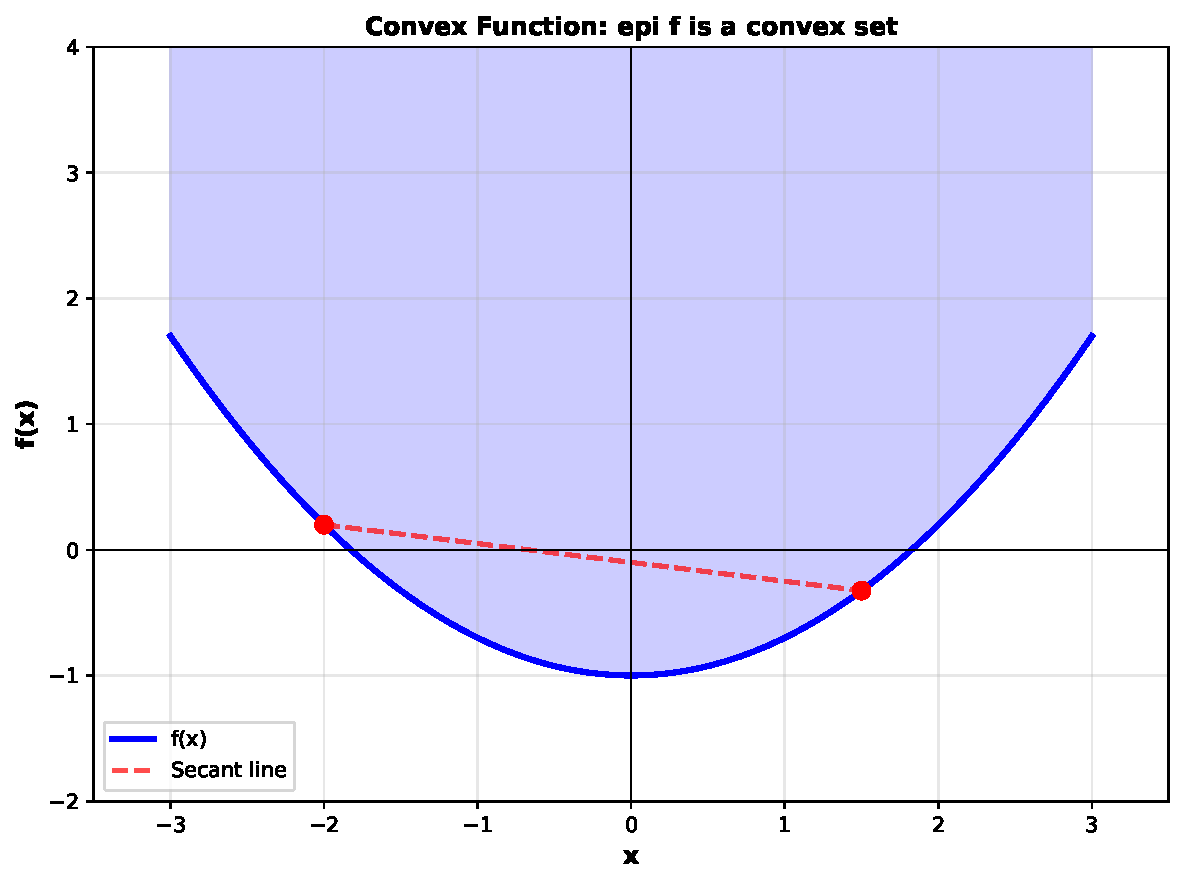
\includegraphics[width=0.8\textwidth]{convex_definition.pdf}
    \end{center}
    
    \textit{The epigraph (shaded region) is convex if and only if the function is convex.}
\end{frame}

\begin{frame}{Strictly Convex vs. Convex}
    \begin{center}
        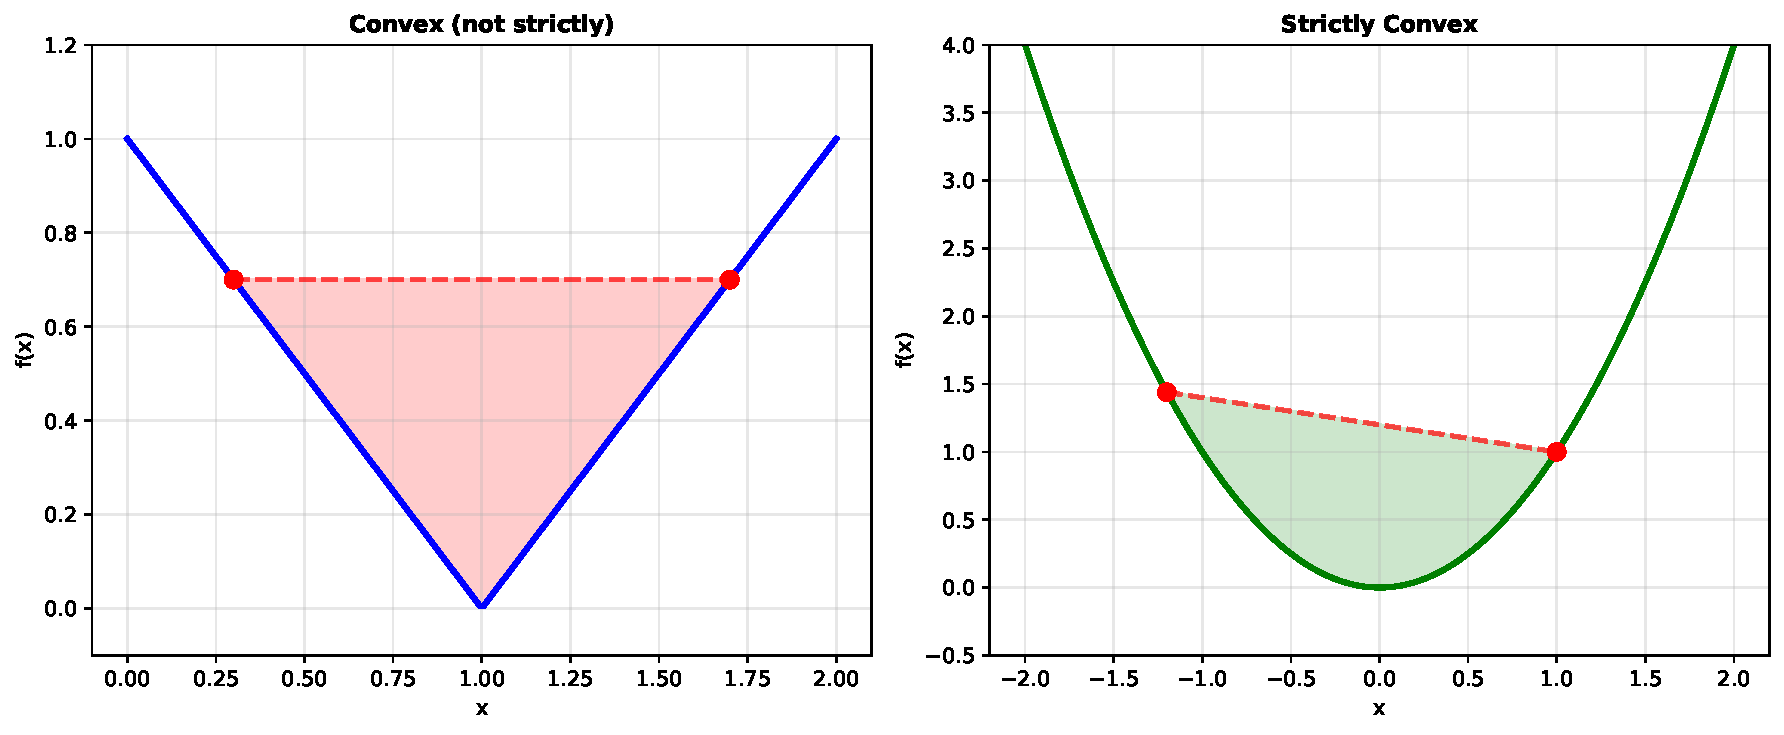
\includegraphics[width=0.95\textwidth]{strictly_convex.pdf}
    \end{center}
    
    \textit{Left: Convex but not strictly (linear segment in graph). Right: Strictly convex (strict inequality).}
\end{frame}

\begin{frame}{Norms and Level Sets}
    \begin{center}
        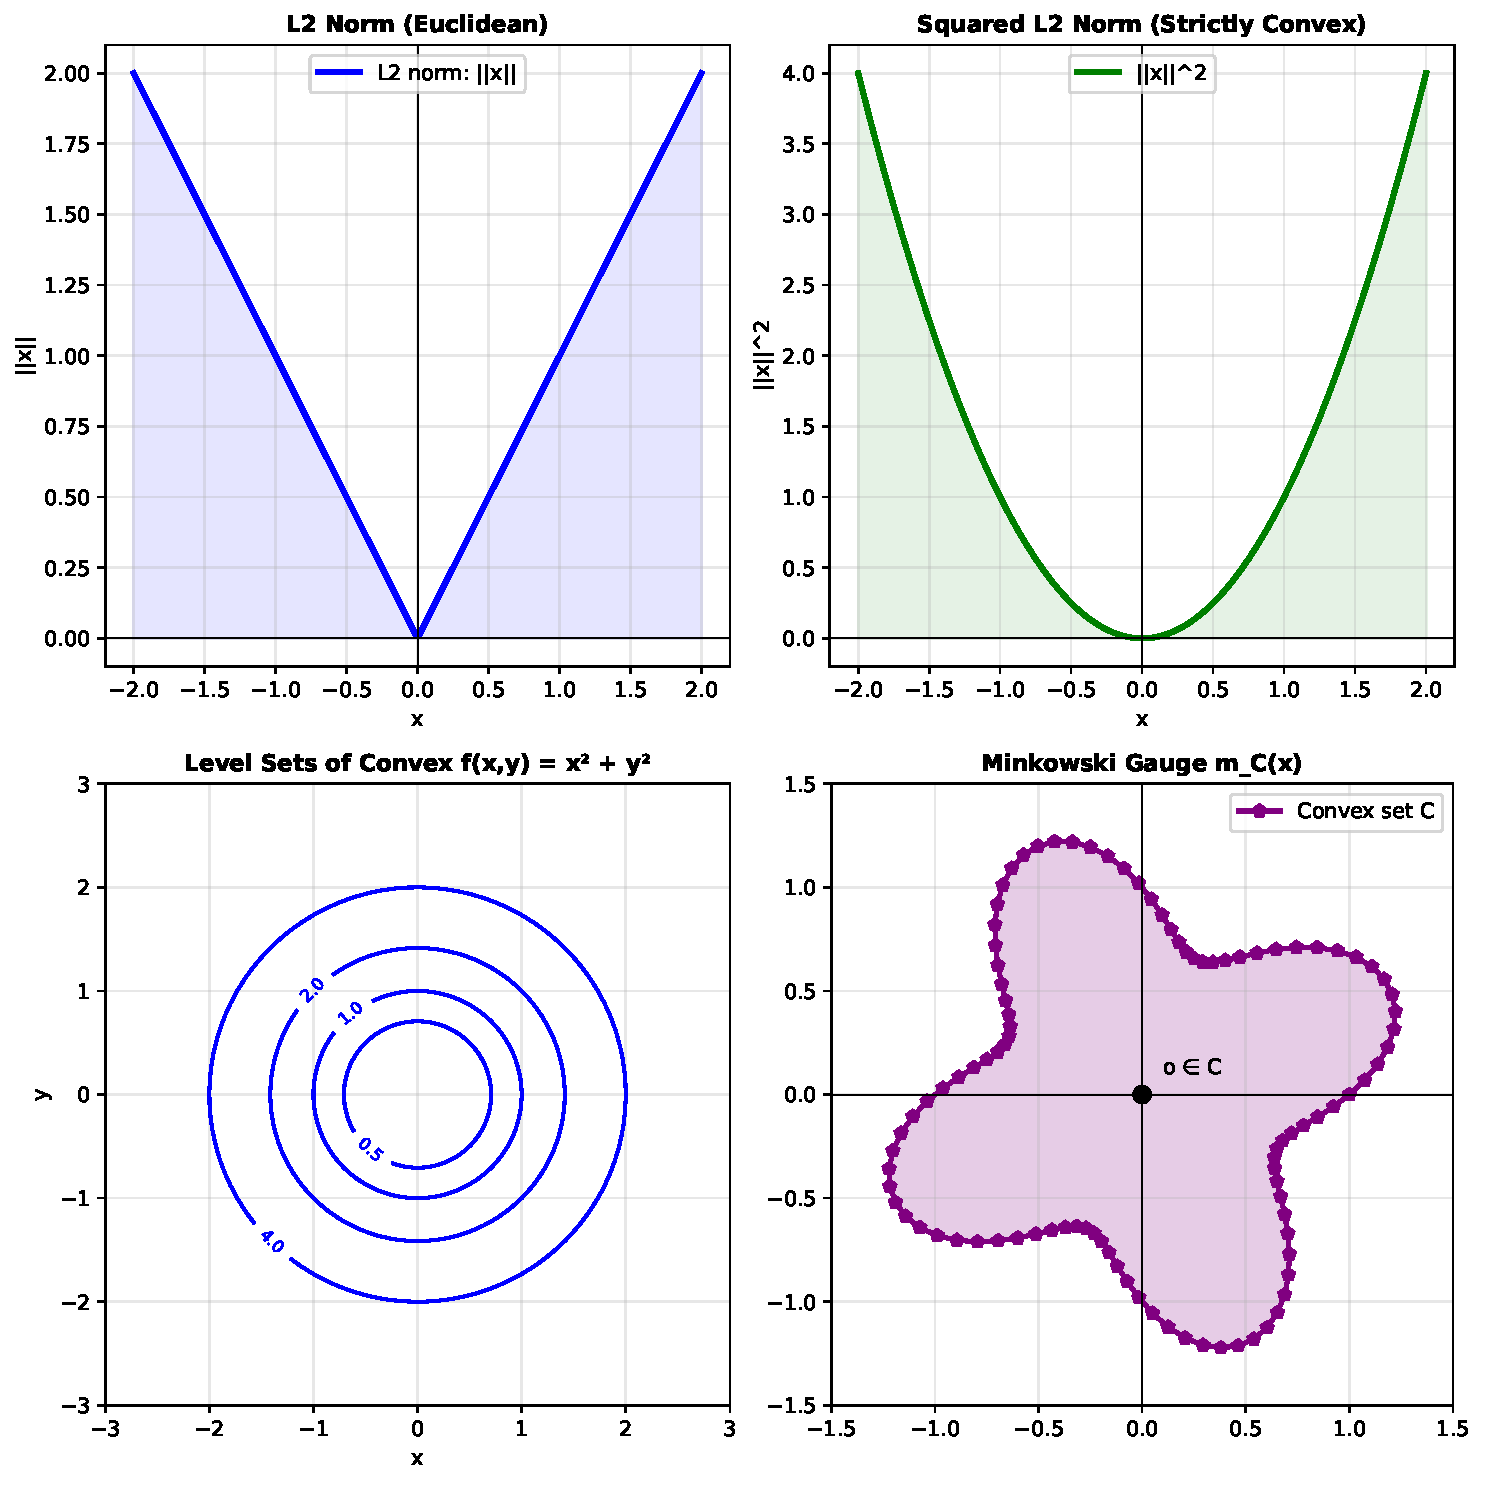
\includegraphics[width=0.95\textwidth]{norms_and_level_sets.pdf}
    \end{center}
\end{frame}

\begin{frame}{Important Divergence Functions}
    \begin{center}
        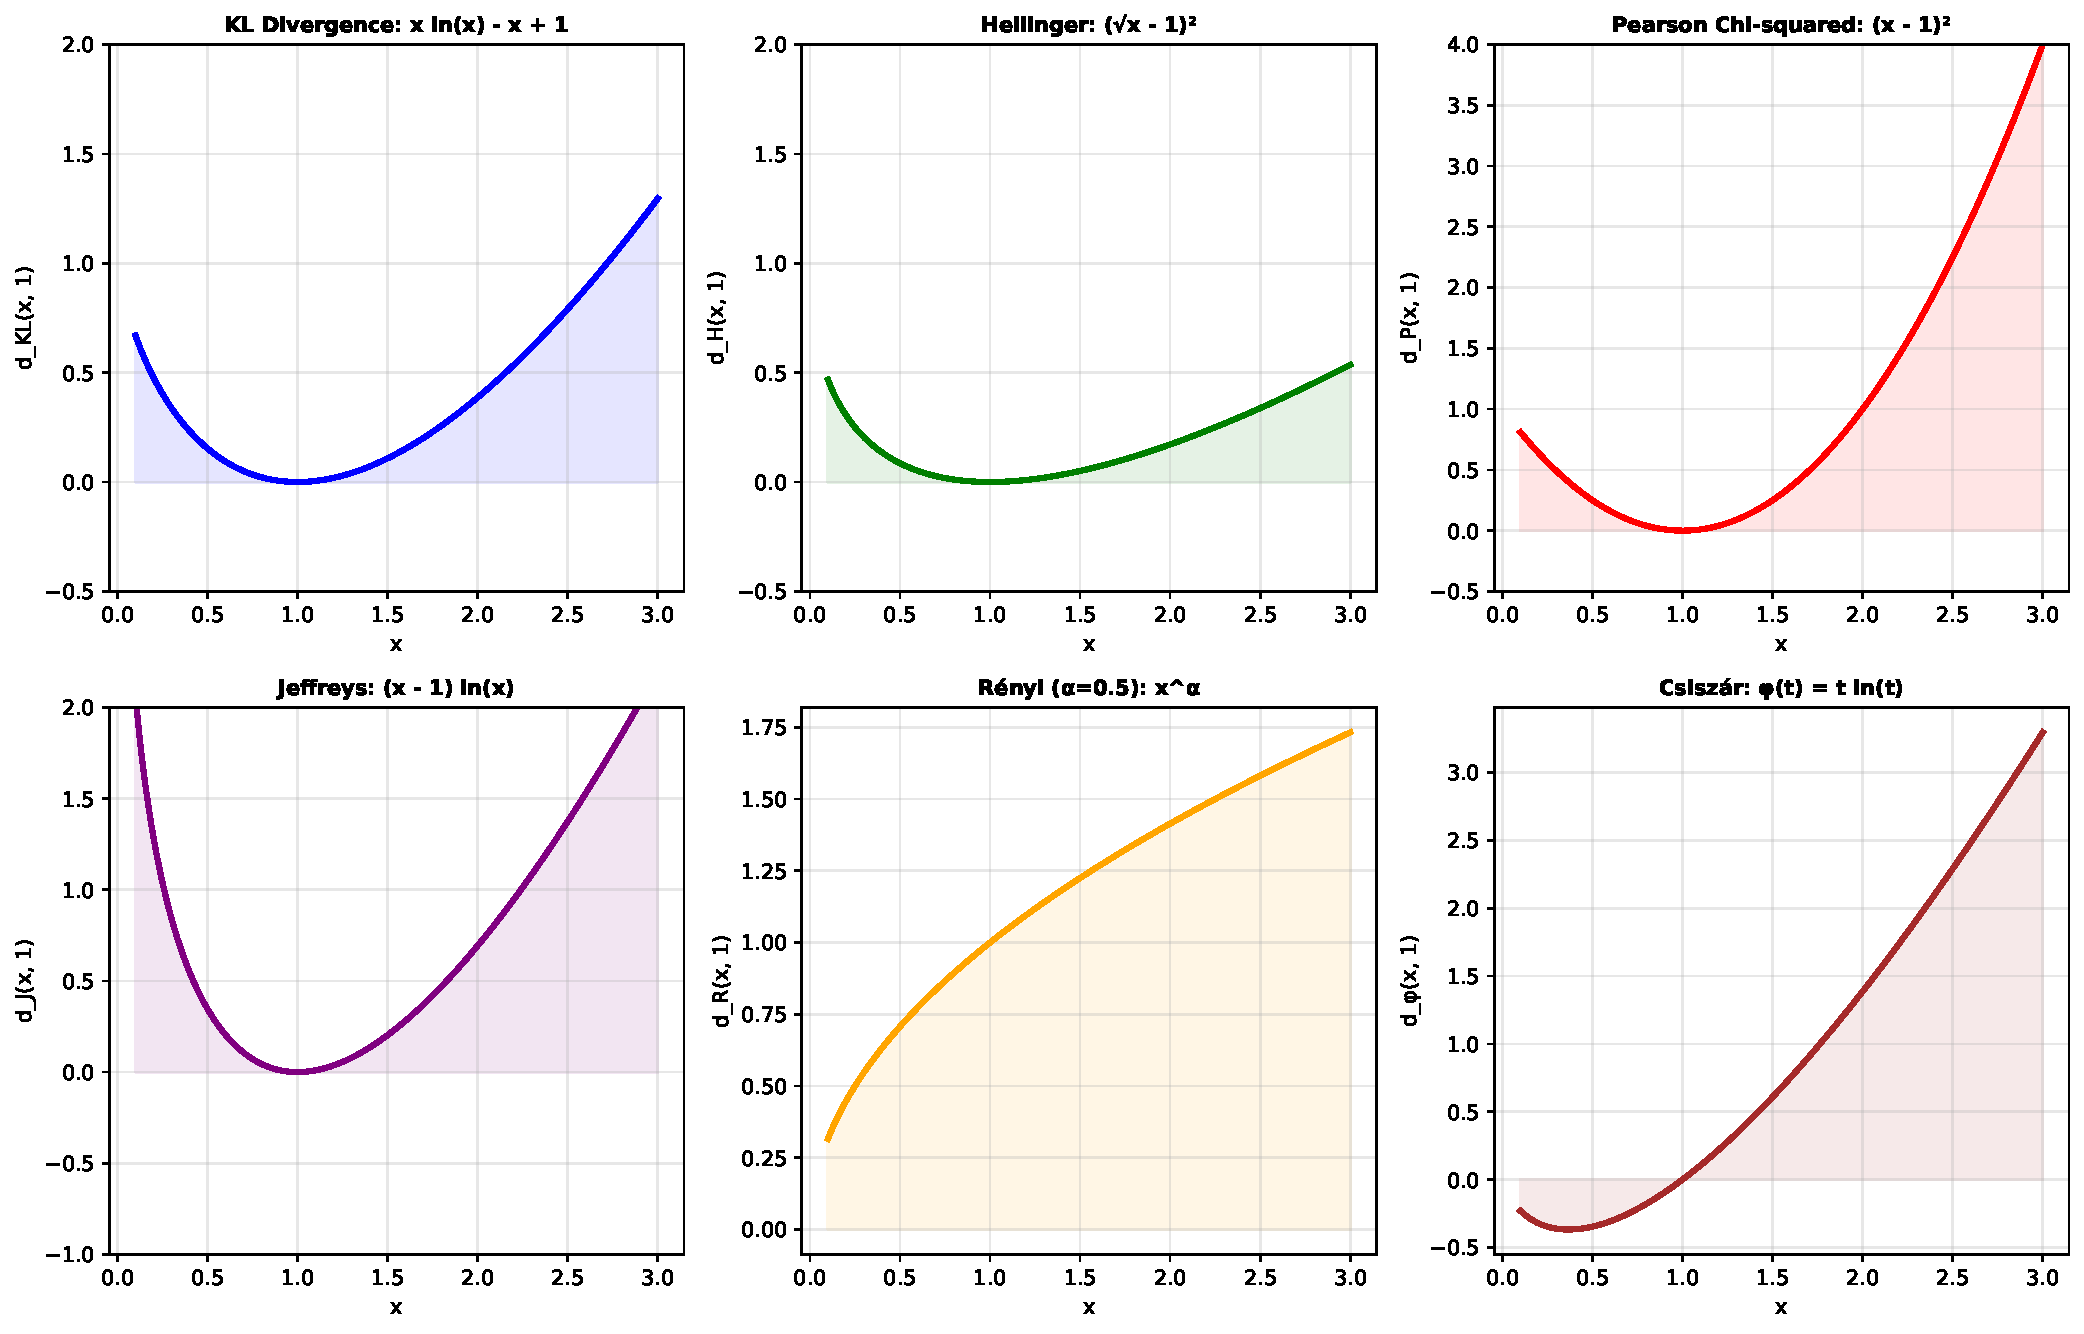
\includegraphics[width=0.95\textwidth]{divergences.pdf}
    \end{center}
    
    \textit{All these divergence measures are convex functions of their first argument.}
\end{frame}

\begin{frame}{Huber Loss Function}
    \begin{center}
        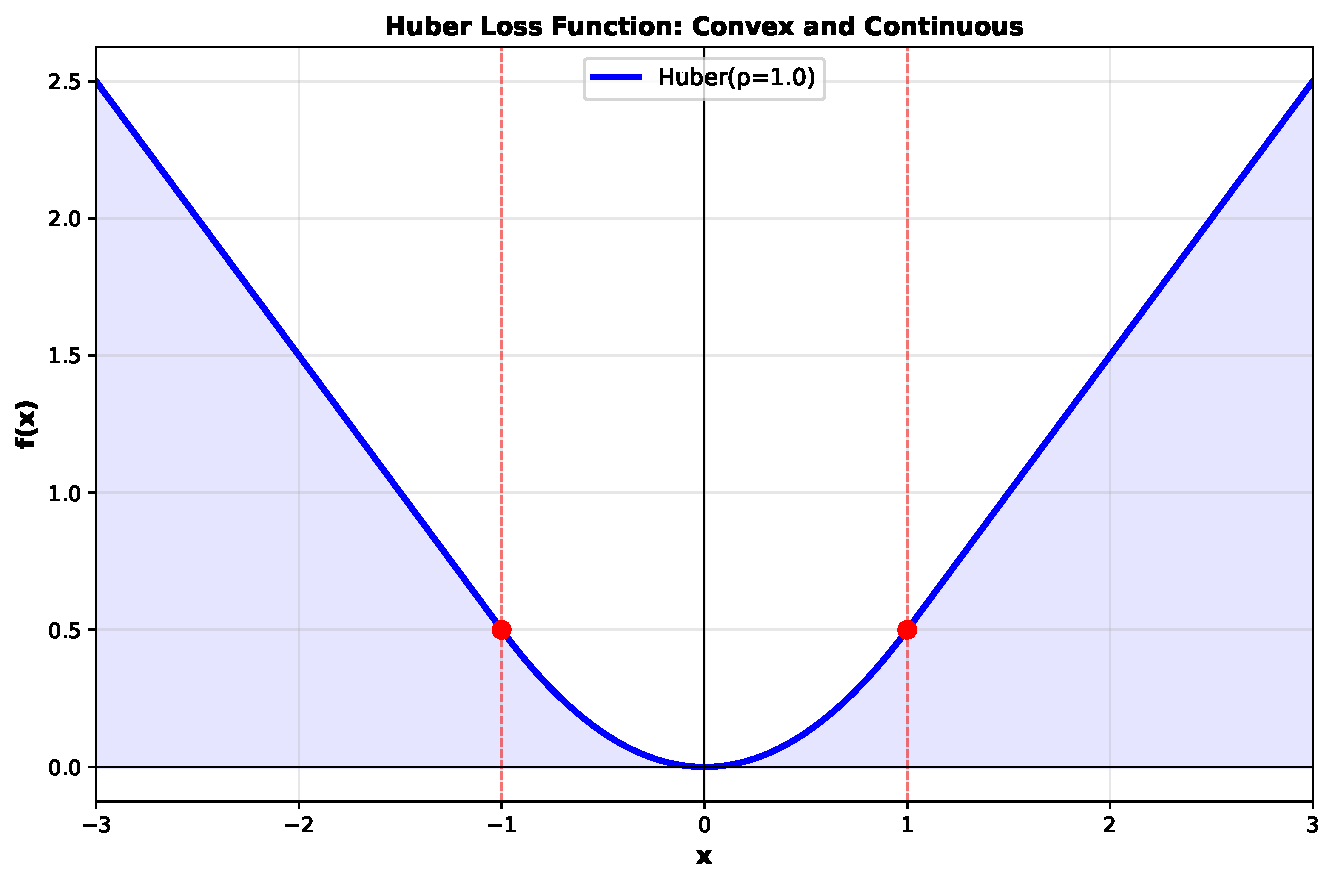
\includegraphics[width=0.8\textwidth]{huber_function.pdf}
    \end{center}
    
    \textit{Combines quadratic loss (near zero) with linear loss (far from zero) -- useful in robust statistics.}
\end{frame}

\begin{frame}{Jensen's Inequality Illustration}
    \begin{center}
        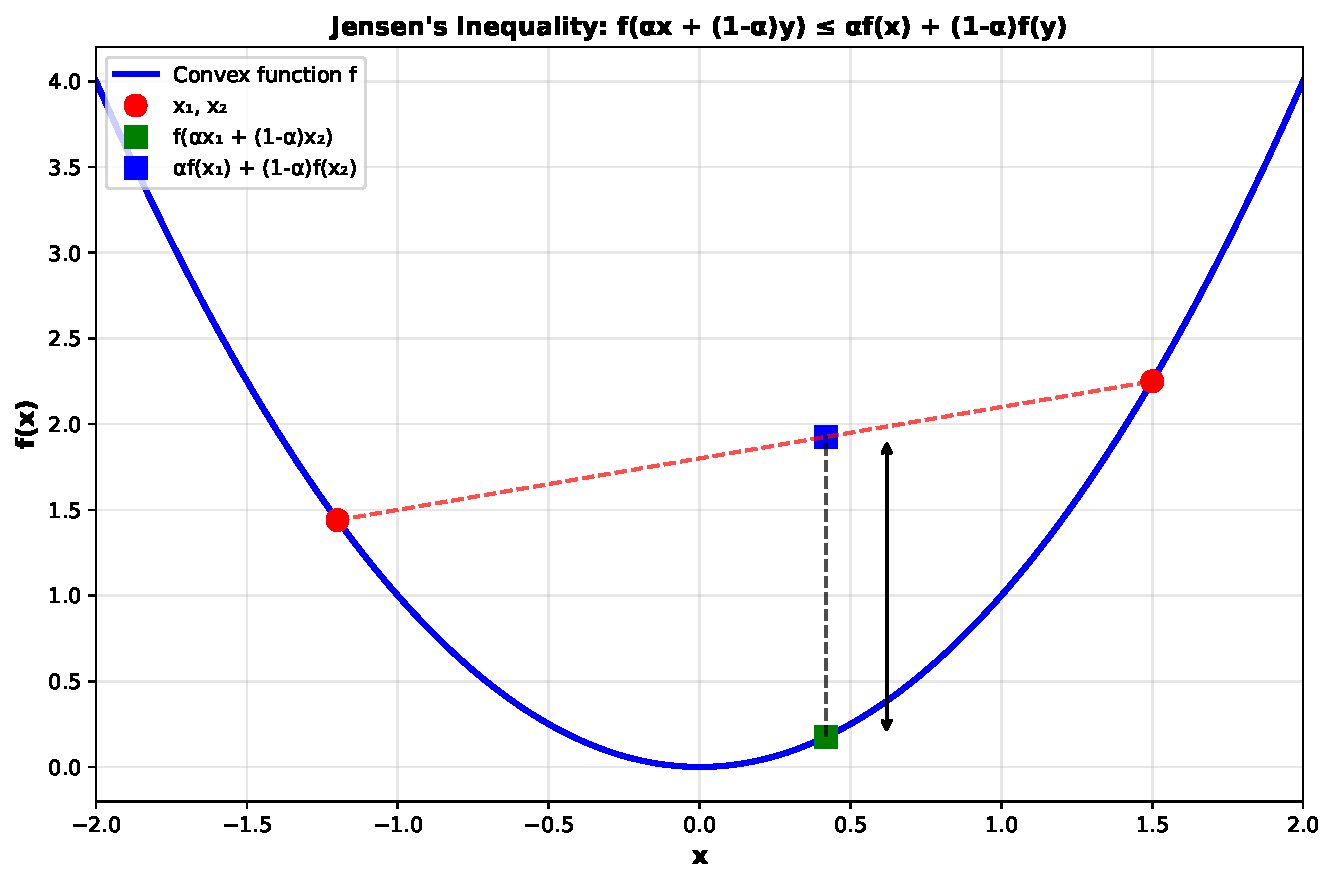
\includegraphics[width=0.8\textwidth]{jensen_inequality.pdf}
    \end{center}
    
    \textit{Function value at weighted average is at most the weighted average of function values.}
\end{frame}

\begin{frame}{Lipschitz Continuity}
    \begin{center}
        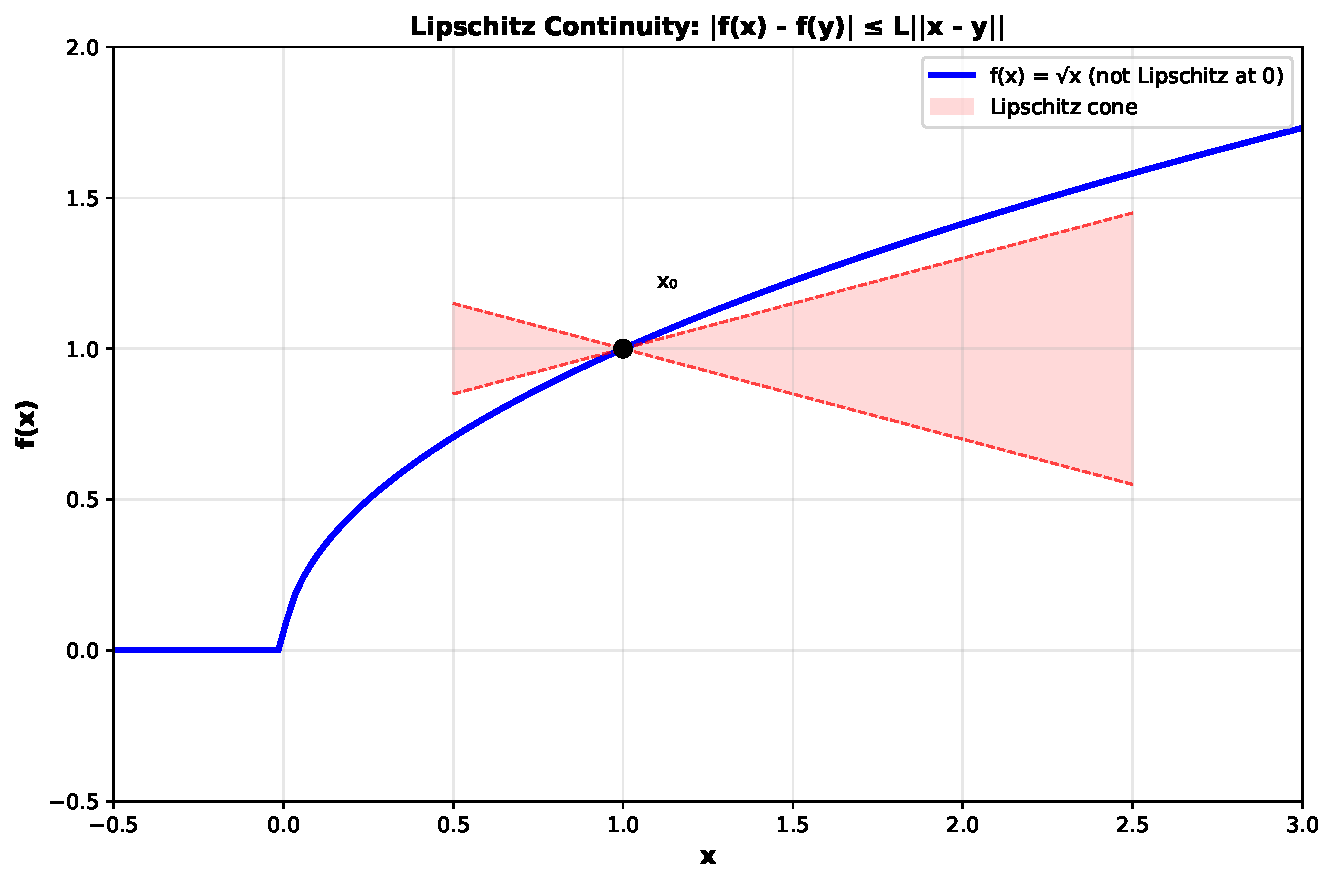
\includegraphics[width=0.8\textwidth]{lipschitz_continuity.pdf}
    \end{center}
    
    \textit{Function stays within a cone of slope $L$ around any point.}
\end{frame}

\begin{frame}{Composition of Convex Functions}
    \begin{center}
        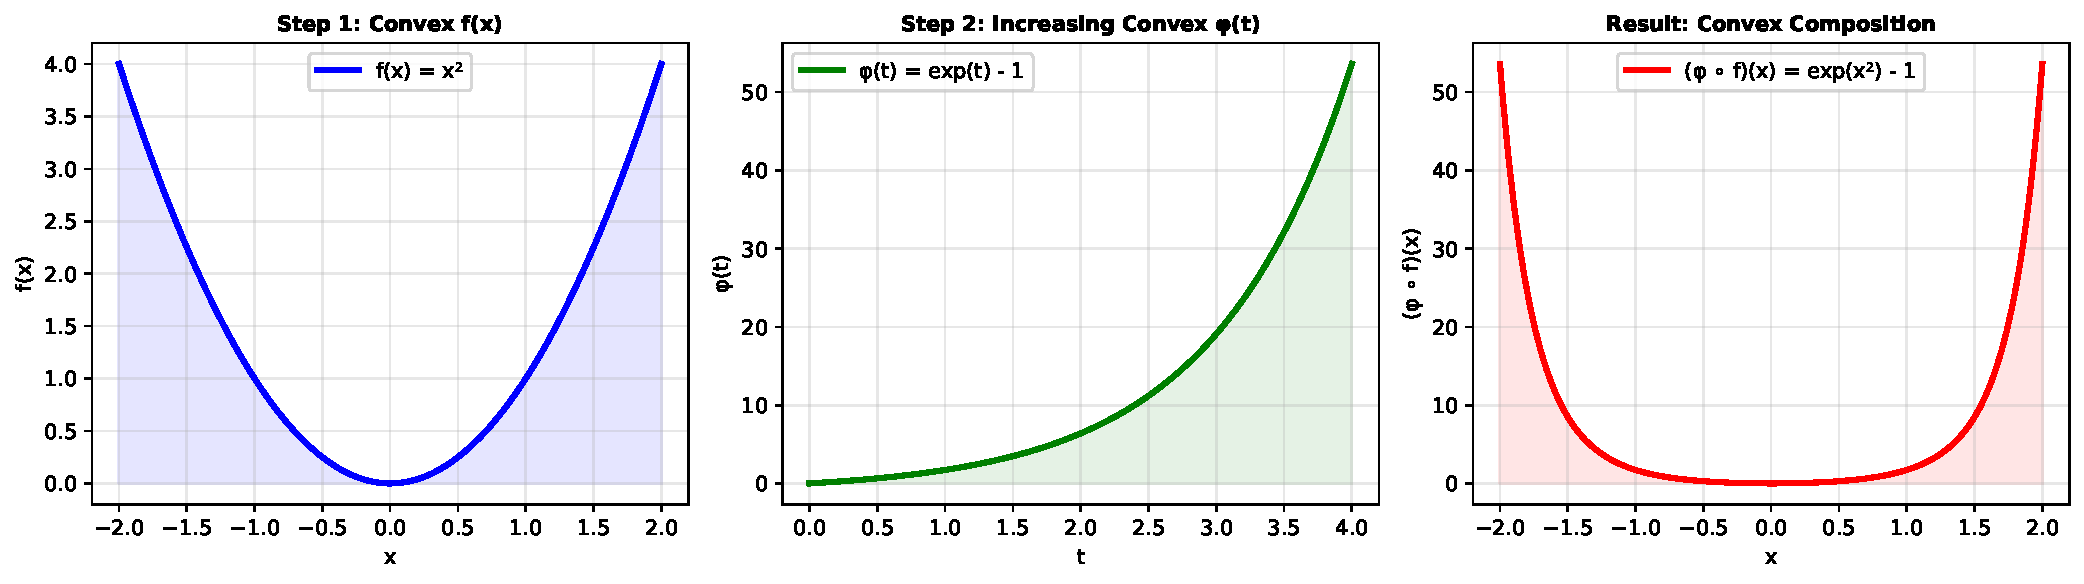
\includegraphics[width=0.95\textwidth]{composition_convex.pdf}
    \end{center}
    
    \textit{Composition of inner convex function $f$ with increasing convex function $\phi$ gives convex result.}
\end{frame}

% ============================================================================
% SUMMARY AND KEY POINTS
% ============================================================================

\section{Summary}

\begin{frame}{Chapter 8: Summary of Key Results}
    \textbf{Core Definitions:}
    \begin{itemize}
        \item Convex functions and their epigraphs
        \item Strictly convex functions
        \item Properties of level sets (convex sets)
    \end{itemize}

    \vspace{0.2cm}

    \textbf{Preservation of Convexity:}
    \begin{itemize}
        \item Supremum of convex functions is convex
        \item Pointwise limits of convex functions are convex
        \item Composition with increasing convex functions preserves convexity
        \item Integrals and perspective functions preserve convexity
    \end{itemize}

    \vspace{0.2cm}

    \textbf{Topological Properties:}
    \begin{itemize}
        \item Boundedness implies Lipschitz continuity
        \item Theorem 8.38: Equivalence of four continuity conditions
        \item In finite dimensions: proper convex functions are continuous on $\text{int dom } f$
    \end{itemize}
\end{frame}

\begin{frame}{Key Inequalities and Examples}
    \textbf{Jensen's Inequality:}
    \[
    f\left(\sum_i \alpha_i x_i\right) \leq \sum_i \alpha_i f(x_i)
    \]

    \vspace{0.3cm}

    \textbf{Norms are convex:} $\|\alpha x + (1-\alpha)y\| \leq \alpha \|x\| + (1-\alpha)\|y\|$

    \vspace{0.3cm}

    \textbf{Squared norms are strictly convex}

    \vspace{0.3cm}

    \textbf{Important Divergences:}
    \begin{itemize}
        \item Kullback-Leibler: $\sum_i p_i \ln(p_i/q_i)$
        \item Jeffreys: $\sum_i (p_i - q_i) \ln(p_i/q_i)$
        \item Hellinger: $\sum_i (\sqrt{p_i} - \sqrt{q_i})^2$
    \end{itemize}

    \vspace{0.2cm}

    \textbf{All are convex in their arguments!}
\end{frame}

\begin{frame}{Applications and Connections}
    \textbf{Optimization:}
    \begin{itemize}
        \item Convex functions have unique global minima (if convex constraints)
        \item Lower semicontinuous convex functions have minimizers in finite-dim spaces
        \item Subdifferential calculus applies (see later chapters)
    \end{itemize}

    \vspace{0.3cm}

    \textbf{Statistics and Machine Learning:}
    \begin{itemize}
        \item Kullback-Leibler divergence: information theory
        \item Huber loss: robust regression
        \item Convex functions: convex optimization problems
    \end{itemize}

    \vspace{0.3cm}

    \textbf{Functional Analysis:}
    \begin{itemize}
        \item Properties of proper convex functions lead to subdifferentials
        \item Connection to weak* lower semicontinuity
    \end{itemize}
\end{frame}

\begin{frame}{Reading Guide}
    \textbf{Essential Results to Master:}
    \begin{enumerate}
        \item Definition 8.1: Convex functions (via convexity of epigraph)
        \item Proposition 8.11: Jensen's inequality
        \item Proposition 8.16--8.18: Preservation under operations
        \item Theorem 8.38: Main continuity theorem
        \item Corollary 8.39--8.41: Finite-dimensional consequences
    \end{enumerate}

    \vspace{0.3cm}

    \textbf{Recommended Exercises:}
    \begin{itemize}
        \item Exercise 8.1--8.5: Basic convexity properties
        \item Exercise 8.10: Arithmetic-geometric mean inequality
        \item Exercise 8.14: Sublevel sets and convexity
        \item Exercise 8.18--8.22: Advanced applications
    \end{itemize}

    \vspace{0.3cm}

    \textbf{Next Chapter (Chapter 9):} Lower Semicontinuous Convex Functions
\end{frame}

\end{document}
